\lecture[7]{Kafli 7: Upphafsgildisverkefni fyrir venjulegar afleiðujöfnur}{lecture-text}
\date{4., 6. og 11.~mars, 2015}

\begin{document}

\section{section}
\begin{frame}
	\maketitle
\end{frame}

\begin{frame}{Yfirlit}
\begin{block}{Kafli 7: Upphafsgildisverkefni fyrir venjulegar afleiðujöfnur}
\begin{center}
\begin{tabular}{|l|l|l|l|}\hline
Kafli &Heiti á viðfangsefni & Bls. & Glærur \\
\hline
7.1 &Almenn atriði um upphafsgildisverkefni & 533-544 & 3-13\\
7.8 & Upphafsgildisverkefni fyrir jöfnuhneppi & 623-631 & 5-8\\
7.2-3 &Aðferð Eulers,  & 546-566 & 14-16\\
7.4 &Runge Kutta aðferðir & 570-578 & 17-26\\
7.6 &Skekkjumat, samleitni og stöðugleiki & 598-607 & 27-28\\
7.7 &Stýring á skekkju og breytileg skrefastærð & 608-621 & 29-37 \\
7.5 &Fjölskrefaaðferðir& 583-594 & 38-46\\
7.6 & Greining á samleitni og stöðugleika&  598-607 & 47-54 \\
\hline
\end{tabular}
\end{center}
\end{block}
\end{frame}
\subsection{subsec}

\begin{frame}{7.1 Almenn atriði} 
\begin{block}{Fyrsta stigs afleiðujafna með upphafsgildi}
\begin{equation*}
\begin{cases}
x' = f(t,x),\\
x(t_0) = x_0.
\end{cases}
\end{equation*}
Hér er gefið fall $f$ á einhverju svæði $U$ í $\mathbb{R}^2$ sem
inniheldur $(t_0,x_0)$. 

\pause
\smallskip
Við segjum að $x$ sé lausn á þessu verkefni ef
$x$ er fall skilgreint á bili $I$, sem er þannig að \pause
\begin{itemize}
 \item $t_0 \in I$, \pause
 \item $(t,x(t)) \in U$ fyrir öll $t \in I$, \pause
 \item $x'(t) = f(t,x(t))$ fyrir öll $t \in I$, og\pause
 \item $x(t_0) = x_0$.
\end{itemize}
\end{block}
\end{frame}


\begin{frame}{7.1 Tilvist og ótvíræðni lausna} 
\begin{equation*}
\begin{cases}
x' = f(t,x)\\
x(t_0) = x_0
\end{cases}
\end{equation*}

Ef $f$ er samfellt, þá er alltaf til lausn á einhverju bili $I$. 
(Setning Peano)

\pause
\smallskip
Ef $f$ uppfyllir Lipschitz-skilyrði með tilliti til $x$, 
þ.e.a.s.~til er fasti $C$ þannig að 
\begin{equation*}
|f(t,x_1) - f(t,x_2)| \leq C|x_1 - x_2|
\end{equation*}
fyrir öll $(t,x_1)$ og $(t,x_2)$ í grennd um $(t_0, x_0)$ þá er
lausnin ótvírætt ákvörðuð. (Setning Picard) 
\end{frame}


\begin{frame}{7.1 Upphafsgildisverkefni fyrir hneppi} 
\begin{equation*}
\begin{cases}
\xv' =\fv(t,\xv)\\
\xv(t_0) = \xv_0
\end{cases}
\end{equation*}

$$
\fv: U \rightarrow \R^n, \qquad U\subset \mathbb{R}^{n+1}, \quad
(t_0,\xv_0) \in U.
$$ 

\pause
\smallskip
Skrifum  $\xv(t)$ og $\fv(t,\xv)$ sem {\it dálkvigra},
$$\xv(t) = [x_1(t), x_2(t), \ldots , x_n(t)]^T
\quad \text{  og } \quad 
\fv(t,\xv) = [f_1(t,\xv), \ldots , f_n(t, \xv)]^T
$$
\end{frame}


\begin{frame}{7.1 Jöfnur af stigi $>1$ og jafngild hneppi}
Jöfnur af hærra stigi má umrita yfir í jafngild hneppi. 
Ef við höfum $m$-stigs diffurjöfnu
\begin{align*}
&u^{(m)} = g(t,u, \ldots , u^{(m-1)})\\
&u(t_0) = u_0, \quad u'(t_0) = u_1, \quad \ldots, \quad  u^{m-1}(t_0) = u_{(m-1)}
\end{align*}
þar sem $g$ er gefið fall og $u_0, \ldots , u_{m-1}$ eru gefnar tölur.

\pause
\smallskip
Jafngilt hneppi er fengið með því að setja 
\begin{align*}
x_1 =& u, \\
x_2 =& u', \\
x_3 =& u'', \\
\vdots& \\
x_m =& u^{(m-1)}
\end{align*}
\end{frame}


\begin{frame}{7.1 Jafngilt hneppi} 
\begin{equation*}
\begin{cases}
x_1' &= x_2 \qquad x_1(t_0) = u_0\\
x_2' &= x_3 \qquad x_2(t_0 = u_1\\
&\vdots \qquad \vdots\\
x_{m-1}' &= x_m \qquad x_m(t_0) = u_{m-1}\\
x_m' &= g(t,x_1, \ldots , x_m)
\end{cases}
\end{equation*}
Lausn hneppisins gefur ótvírætt lausn á upprunalegu $m$-ta stigs 
afleiðujöfnunni.
\end{frame}


\begin{frame}{7.1 Tilvist og ótvíræðni lausna á hneppum} 
Tilvistar- og ótvíræðnisetningar Peanos og  Picards 
eru þær sömu fyrir hneppi

\begin{equation*}
\begin{cases}
\xv' =\fv(t,\xv)\\
\xv(t_0) = \xv_0
\end{cases}
\end{equation*}

\pause
\smallskip
Við þurfum bara að 
setja norm $\|\cdot\|$ í stað tölugildis $|\cdot|$ í öllum ójöfnum og
þar með talið í Lipschitz-skilyrðinu.
\end{frame}


\begin{frame}{7.1 Ritháttur} 
Til einföldunar á rithætti skulum við skrifa lausnarvigurinn $\xv$ 
og vörpunina $\fv$ sem $x$ og $f$ og láta eins og við séum að leysa 
fyrsta stigs afleiðujöfnu.

\pause
\smallskip
Við veljum gildi $t_0 < t_1 < \cdots < t_j<\cdots$ og reiknum út
nálgunargildi $w_j$ á gildi lausnarinnar $x(t_j)$ í punktinum
$t_j$.   Gildið $w_0=x(t_0)$ er rétta upphafsgildi lausnarinnar 

\smallskip
Talan $t_j$ kallast $j$-ti tímapunkturinn og talan
$h_j=t_j-t_{j-1}$ nefnist $j$-ta tímaskrefið.
\end{frame}


\begin{frame}{7.1 Heildum lausnina}
Ef við heildum lausn afleiðujöfnunnar yfir tímabilið 
$[t,t+h]$, þá fáum við að hún uppfyllir jöfnuna
$$
x(t+h)=x(t)+\int_t^{t+h}f(\tau,x(\tau))\, d\tau
=x(t)+h\int_0^1f(t+sh,x(t+sh))\, ds.
$$

\pause
\smallskip
Ef við setjum $t=t_{j-1}$ inn í þessa jöfnu, þá fáum við
$$
\dfrac{x(t_j)-x(t_{j-1})}{h_j}=\int_0^1f(t_{j-1}+sh_j,x(t_{j-1}+sh_j))\, ds
$$
\end{frame}


\begin{frame}{7.1 Almennt um nálgunaraðferðir} 
Við leggjum til grundvallar jöfnuna
$$
  \dfrac{x(t_j)-x(t_{j-1})}{h_j}=\int_0^1f(t_{j-1}+sh_j,x(t_{j-1}+sh_j))\, ds
$$
Nálgunaraðferðirnar snúast allar um að gera einhvers konar nálgun á
heildinu í hægri hliðinni
$$
  \int_0^1f(t_{j-1}+sh_j,x(t_{j-1}+sh_j))\, ds
  \approx \varphi(f,t_0,\dots,t_j,w_0,\dots,w_j)
$$
og leysa síðan $w_j$ út úr jöfnunni 
$$
  \dfrac{w_j-w_{j-1}}{h_j}=\varphi(f,t_0,\dots,t_j,w_0,\dots,w_j)
$$
\end{frame}


\begin{frame}{7.1 Beinar og óbeinar aðferðir} 
Nálgunaraðferð sem byggir á jöfnunni
$$
  \dfrac{w_j-w_{j-1}}{h_j}=\varphi(f,t_{0},\dots,t_j,w_{0},\dots,w_j)
$$
er nefnist {\it bein aðferð} (e.~explicit method) ef 
$w_j$ kemur ekki fyrir í í hægri hliðinni.  

\smallskip
Annars nefnist hún  {\it óbein aðferð} eða {\it fólgin aðferð} 
(e.~implicit method).

\smallskip
Ef aðferðin er bein og við höfum reiknað út $w_0,\dots,w_{j-1}$,
þá fáum við rakningarformúlu, þannig að 
$w_j\approx x(t_j)$ er reiknað út
$$
  w_j=w_{j-1}+h_j\varphi(f,t_{0},\dots,t_j,w_{0},\dots,w_{j-1})
$$
\end{frame}


\begin{frame}{7.1 Eins skrefs aðferðir og fjölskrefaaðferðir} 
Nálgunaraðferð sem byggir á jöfnunni
$$
  \dfrac{w_j-w_{j-1}}{h_j}=\varphi(f,t_{j-1},t_j,w_{j-1},w_j)
$$
er nefnist {\it eins skrefs aðferð} (e.~one step method) og er þá
vísað til þess að fallið í hægri hliðinni er einungis háð gildum á
síðasta tímaskrefinu.

\pause
\smallskip
{\it Tveggja skrefa aðferð} er af gerðinni
$$
  \dfrac{w_j-w_{j-1}}{h_j}=\varphi(f,t_{j-2},t_{j-1},t_j,w_{j-2},w_{j-1},w_j)
$$

\pause
\smallskip
Almennt er {\it $k$-skrefa aðferð} af gerðinni
$$
\dfrac{w_j-w_{j-1}}{h_j}=\varphi(f,t_{j-k},\dots,t_j,w_{j-k},\dots,w_j)
$$
{\it Fjölskrefaðferð} er  $k$-skrefa aðferð með $k\geq 2$.
\end{frame}


\begin{frame}{7.2 Aðferð Eulers} 
Rifjum upp að lausnin uppfyllir
\begin{align*}
  x(t+h) - x(t) &= \int\limits_t^{t+h} x'(\tau) \, d\tau
  = \int\limits_t^{t+h} f(\tau,x(\tau)) \, d\tau\\
&= h\int\limits_0^{1} f(t+sh,x(t+sh)) \, ds
\end{align*}

\pause
\smallskip
Billengdin í síðasta heildinu er $1$, svo við 
tökum einföldustu nálgum sem hugsast getur 
en það er gildið í vinstri endapunkti
$f(t,x(t))$.   Fyrir lítil $h$ fæst því 
\begin{equation*}
  x(t+h) \approx x(t) + hf(t,x(t)).
\end{equation*}

\pause
\smallskip
Við þekkjum $w_0=x(t_0)$, svo með þessu getum við fikrað okkur áfram
og  fengið runu nálgunargilda $w_0, w_1, w_2, \ldots$ þannig að
\begin{equation*}
  w_j = w_{j-1} + h_{j} f(t_{j-1},w_{j-1}).
\end{equation*}
\end{frame}


\begin{frame}[fragile]{7.2 Matlab forrit fyrir aðferð Eulers} 
\begin{verbatim}
function w = euler(f,t,alpha);  
%   function w = euler(f,t,alpha) 
% Aðferð Eulers fyrir afleiðujöfnuhneppi 
%         x'(t)=f(t,x(t)), x(0)=alpha. 
% Inn fara: f - fallið f 
%           t - vigur með skiptingu á t-ás. 
%           alpha - upphafsgildið í t(1). 
% Út koma:  w - fylki með nálgunargildunum. 

N = length(t);   
m = length(alpha); 
w = zeros(m,N);  
w(:,1) = alpha; 
for j=2:N 
   w(:,j) = w(:,j-1)+(t(j)-t(j-1))*f(t(j-1),w(:,j-1));
end 
\end{verbatim}
\end{frame}

\begin{frame}[fragile]{7.2. Aðferð Eulers prófuð}
Prófum aðferð Eulers á afleiðujöfnunni
$$
  x' = \frac tx, \qquad x(0) = 1
$$
Við sjáum að rétt lausn er $x(t) = \sqrt{t^2+ 1}$.\pause

Notum 101 jafndreifð tímagildi á bilinu [0,5]. Þá er skekkjan
 \begin{verbatim}
 >> f = @(t,x) t./x;  t=linspace(0,5,101);
 >> w=euler(f,t,1);   plot(t,sqrt(t.^2+1) - w)
 \end{verbatim}

\mode<presentation>
{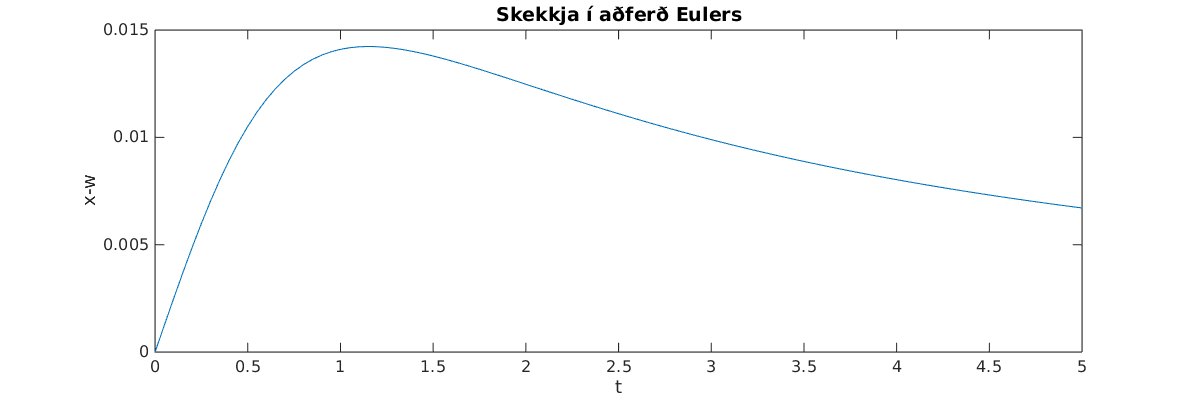
\includegraphics[width=11cm]{./7euler.png}}
\mode<article>
{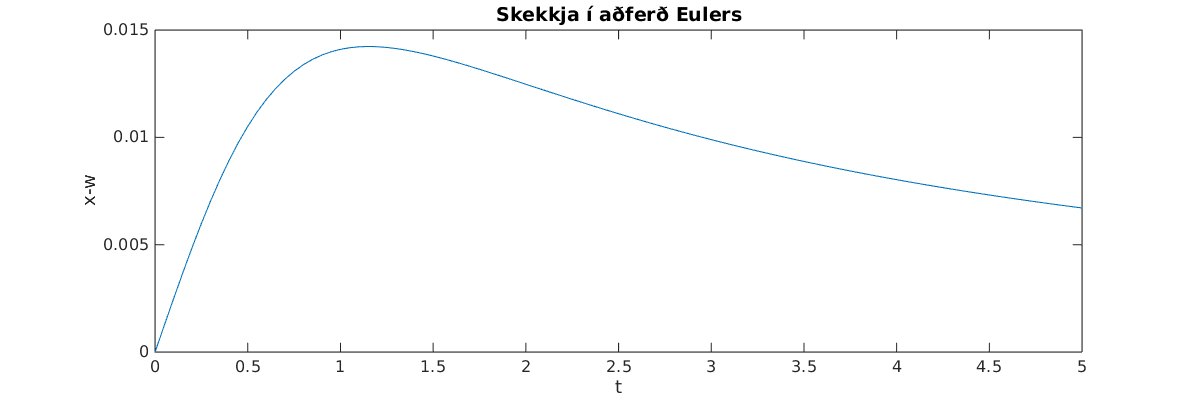
\includegraphics[width=17cm]{./7euler.png}}
\end{frame}


\begin{frame}{7.4 Runge-Kutta aðferðir  -- Aðferð Eulers endurbætt} 
Í aðferð Eulers nálguðum við heildið $\int_0^1 f(t+sh,x(t+sh))\, ds$
með margfeldi af billengdinni og fallgildinu í vinstri endapunkti.

\smallskip
Við getum endurbætt þessa nálgun með því að taka 
einhverja nákvæmari tölulega nálgun á heildinu til dæmis 
miðpunktsaðferð 

\pause
\smallskip
Nálgunarformúlan verður þá
$$
\int_0^1f(t+sh,x(t+sh))\, ds \approx f(t+\tfrac 12h,x(t+\tfrac 12 h)). 
$$
Nú er vandamálið að við höfum nálgað $x(t_{j-1})$ með $w_{j-1}$ en
höfum ekkert nálgunargildi á $x(t_{j-1}+\frac 12 h_j)$.  

\pause
\smallskip 
Við grípum þá til
fyrsta stigs Taylor nálgunar
\begin{align*}
x(t_j+\tfrac 12 h_j)&=x(t_{j-1})+x'(t_{j-1})\big(\tfrac 12 h_j \big)
+\tfrac 12x''(\xi)\big(\tfrac 12 h_j \big)^2\\
&\approx w_{j-1}+\tfrac 12 h_jf(t_{j-1},w_{j-1}).
\end{align*}
\end{frame}


\begin{frame}{7.4 Aðferð Eulers endurbætt} 
Endurbætt aðferð Eulers er þá í tveim skrefum; við
reiknum 
\begin{equation*}
  \tilde w_j = w_{j-1} + \tfrac 12 h_j f(t_{j-1},w_{j-1})
\end{equation*}
og fáum svo nálgunargildið
\begin{equation*}
  w_j = w_{j-1} + h_jf\left(
    t_{j-1}+\tfrac 12 h_j,\tilde w_j\right)
\end{equation*}
\end{frame}


\begin{frame}{7.4 Annað afbrigði af aðferð Eulers -- Aðferð Heun} 
Lítum nú á aðra aðferð þar sem við nálgum heildið með trapisuaðferð. 
$$
\int_0^1f(t+sh,x(t+sh))\, ds \approx 
\tfrac 12 \big(f(t,x(t))+f(t+h,x(t+h))\big). 
$$

\pause
\smallskip
Af þessu leiðir að nálgunarformúlan á að vera
$$
w_j=w_{j-1}+\tfrac 12h_j\big(f(t_{j-1},w_{j-1})+f(t_j,w_j)\big)
$$

\pause
Þetta er greinilega óbein aðferð svo við verðum að byrja á 
nálgun á $w_j$, með
$$
w_j\approx x(t_j)=x(t_{j-1}+h_j)\approx x(t_{j-1})+h_jx'(t_{j-1})
=x(t_{j-1})+h_jf(t_{j-1},w_{j-1}) 
$$

\smallskip
Þetta nýja afbrigði af aðferð Eulers nefnist {\it aðferð Heun}.
Hún er í tveim skrefum:  Við reiknum fyrst
\begin{equation*}
  \tilde w_j = w_{j-1} + h_jf(t_{j-1},w_{j-1})
\end{equation*}
og fáum svo nálgunargildið
\begin{equation*}
  w_j = w_{j-1} + \tfrac 12h_j
\big(f(t_{j-1},w_{j-1})+f(t_j,\tilde w_j)\big)
\end{equation*}
\end{frame}


\begin{frame}{7.4 Forsagnar- og leiðréttingaraðferð} 
Endurbætt aðferð  Eulers og  aðferð Heun eru leiðir til þess að vinna
úr óbeinum aðferðum, þar sem rakningarformúlan fyrir nálgunargildin er
af gerðinni
$$
w_j=w_{j-1}+h_j\varphi(f,t_{j-1},t_j,w_{j-1},w_j)
$$
og okkur vantar eitthverja nálgun á $w_j$ til þess að stinga inn í
hægri hlið þessarar jöfnu.  Við skiptum þessu tvö skref:

\pause
\smallskip
{\bf Forsagnarskref:}   Við beitum einhverri beinni aðferð til þess að
reikna út 
$$
\tilde w_j=w_{j-1}+h_j\psi(f,t_{j-1},t_j,w_{j-1})
$$

\pause
\smallskip
{\bf Leiðréttingarskref:} Setjum
$$
w_j=w_{j-1}+h_j\varphi(f,t_{j-1},t_j,w_{j-1},\tilde w_j).
$$
\end{frame}


\begin{frame}{7.4 2.~stigs Runge-Kutta-aðferð} 
Lítum aftur á verkefnið
\begin{equation*}
  \left\{
    \begin{array}{l}
      x'(t) = f(t,x(t)) \\
      x(t_0) = x_0
    \end{array}
  \right.
\end{equation*}
og skoðum 2. stigs Taylor liðun á lausninni $x$ í punkti
$t$. Innleiðum fyrst smá rithátt til styttingar, setjum 
\begin{equation*}
  x = x(t), \quad f'_t = \frac{\partial f}{\partial t}(t,x(t)), \quad
  f = f(t,x(t)), \quad f'_x = \frac{\partial f}{\partial x}(t,x(t)).
\end{equation*}
Keðjureglan gefur
$$
x''(t)=\dfrac d{dt}f(t,x(t))=f'_t+f'_xx'(t)=f'_t+f\,f'_x.
$$
\end{frame}


\begin{frame}{7.4 2.~stigs Runge-Kutta-aðferð} 
Taylor-liðun lausnarinnar er 
\begin{align*}
  x(t+h) &= x + hx'(t) + \frac{1}{2} h^2 x''(t) + O(h^3) \\
  &= x + hf + \frac{1}{2} h^2 ( f'_t + f f'_x ) + O(h^3) \\
  &= x + \frac{1}{2}hf + \frac{1}{2}h( f + hf'_t + (hf)f'_x) + O(h^3)
\end{align*}
Nú sjáum við að síðasti liðurinn er 1. stigs Taylor 
liðun $f$ með miðju $(t,x)$ skoðuð í punktinum $(t+h,x+hf)$, því
\begin{equation*}
  f(t+h,x + hf) = f + hf'_t + (hf) f'_x + O(h^2)
\end{equation*}
og þar með er
\begin{equation*}
  x(t+h) = x(t) + \frac{1}{2} hf(t,x) + \frac{1}{2} hf(t+h,x+hf) + O(h^3)
\end{equation*}
\end{frame}


\begin{frame}{7.4 2.~stigs Runge-Kutta-aðferð} 
Við höfum leitt út
\begin{equation*}
  x(t+h) = x(t) + \tfrac{1}{2} hf(t,x) + \tfrac{1}{2} hf(t+h,x+hf) + O(h^3)
\end{equation*}
Þessi formúla liggur til grundvallar 
2.~stigs Runge-Kutta-aðferð:
Með henni fáum við nálgunarrunu $w_0, w_1, w_2, \ldots$ þannig að
$w_0=x(0)$ og 
\begin{equation*}
  w_j = w_{j-1} + \tfrac{1}{2}(F_1 + F_2), \quad j = 1,2,\ldots
\end{equation*}
þar sem
\begin{equation*}
  F_1 = h_jf(t_{j-1},w_{j-1}),
  \quad \text{og} \quad
  F_2 = h_jf(t_j,w_{j-1}+F_1)
\end{equation*}
og eins og alltaf er $w_j \approx x(t_j)$.
\end{frame}


\begin{frame}[fragile]{7.4 Matlab forrit fyrir 2.~stigs Runge-Kutta-aðferð} 
\begin{verbatim}
function w = runge_kutta_2(f,t,alpha);
%   w = runge_kutta_2(f,t,alpha)
% 2. stigs Runge-Kutta aðferð fyrir afleiðuhneppi 
%         x'(t)=f(t,x(t)), x(0)=alpha. 
% Inn fara: f - fallið f 
%           t - vigur með skiptingu á t-ás. 
%           alpha - upphafsgildið í t(1). 
% Út koma:  w - fylki með nálgunargildunum. 
N = length(t);   
m = length(alpha); 
w = zeros(m,N);  
w(:,1) = alpha; 
for j=2:N 
  h = t(j)-t(j-1);
  F1 = h*f(t(j-1),w(:,j-1));
  F2 = h*f(t(j),w(:,j-1)+F1); 
  w(:,j) = w(:,j-1) + (F1+F2)/2; 
end 
\end{verbatim}
\end{frame}

\begin{frame}{7.4 Klassíska fjórða stigs Runge-Kutta aðferðin}
 Algengasta Runge-Kutta aðferðin er klassíska Runge-Kutta aðferðin. Þetta
 er fjórða stigs aðferð, sem þýðir að staðarskekkjan er $O(h^5)$ og heildarskekkjan er $O(h^4)$.
\pause
$$
 w_{j} = w_{j-1} + \frac 16(k_1 + 2k_2 + 2k_3 + k_4),
 $$
 \pause
 þar sem
 \begin{align*}
  k_1 &= hf(t_{j-1},w_{j-1}) \\
  k_2 &= hf\left(t_{j-1} + \frac h2,w_{j-1}+ \frac{k_1}2\right) \\
  k_3 &= hf\left(t_{j-1} + \frac h2,w_{j-1}+ \frac{k_2}2\right) \\
  k_4 &= hf(t_{j-1} + h,w_{j-1}+ k_3).
 \end{align*}
 
 \pause
 Ef $f(t,x)$ er bara fall af $t$, þ.e.~óháð $x$, þá svarar þetta til þess að meta heildið $\phi$
 með Simpson-reglunni.

\end{frame}

\begin{frame}[fragile]{7.4 Runge-Kutte 4 prófuð}
Skoðum nú sama dæmi og þegar við prófuðum aðferð Eulers.

Þá gefa eftirfarandi skipanir mynd af skekkjunni.
\begin{verbatim}
>> f = @(t,x) t./x;
>> [w,t]=rk4(f,0,1,5,100);
>> plot(t,sqrt(t.^2+1) - w)
\end{verbatim}

\mode<presentation>
{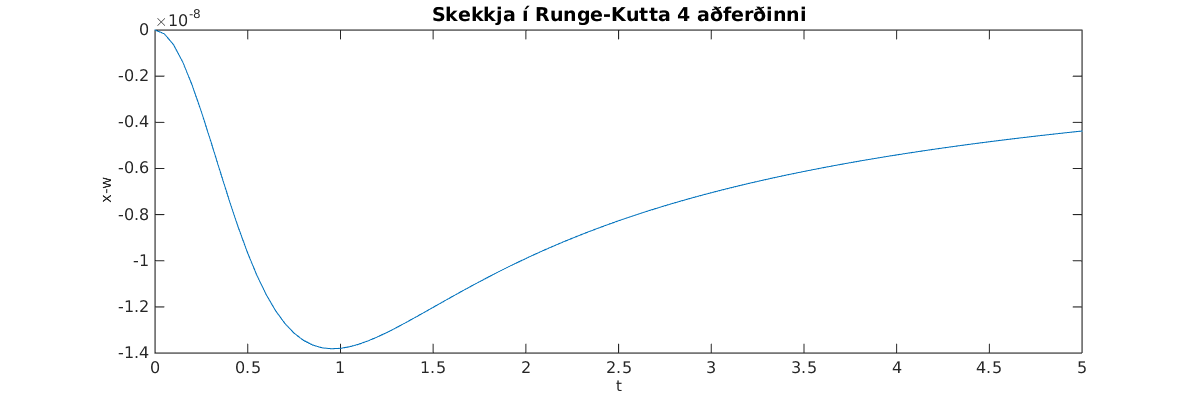
\includegraphics[width=11cm]{./7rk4.png}}
\mode<article>
{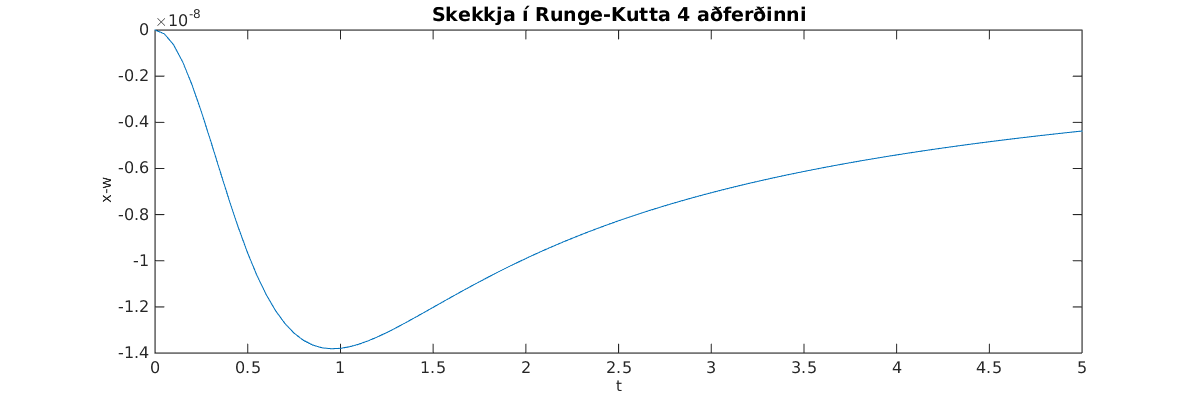
\includegraphics[width=17cm]{./7rk4.png}}
\end{frame}


\begin{frame}{7.6 Skekkjumat, samleitni og stöðugleiki} 
Fyrir eins skrefs aðferð skilgreinum við {\it staðarskekkju}
við tímann $t_n$ sem
$$ 
\tau_n = \dfrac{x(t_n)-x(t_{n-1})}{h_n} - 
\varphi(f,t_{n-1},t_n,x(t_{n-1}),x(t_{n})) 
$$

\pause
\smallskip
Hér er réttu lausninni stungið inn í nálgunarformúluna.
Munum að hún uppfyllir 
$$
\dfrac{x(t_n)-x(t_{n-1})}{h_n}
=\int_0^1 f(t_{n-1}+sh_n,x(t_{n-1}+sh_n))\, ds
$$

\pause
\smallskip
Viljum geta metið $\tau_n$ sem fall af $h_n$, t.d.
  $$ 
    \tau_n = O(h_n^k) 
  $$

\pause
\smallskip
Almennt batna aðferðir eftir því sem veldisvísirinn  $k$ 
í staðarskekkjunni verður stærri.
\end{frame}


\begin{frame}{7.6 Staðarskekkja í aðferð Eulers} 
Aðferð Eulers er sett fram með formúlunni
$$
  w_n=w_{n-1}+h_nf(t_{n-1},w_{n-1})
$$ 

\pause
Staðarskekkjan er því
\begin{align*}
  \tau_n&=\dfrac{x(t_n)-x(t_{n-1})}{h_n}-f(t_{n-1},x(t_{n-1}))\\
&=\dfrac{x(t_n)-x(t_{n-1})-x'(t_{n-1})h_n}{h_n}\\
&=\dfrac{\tfrac 12 x''(\xi_{n})h_{n-1}^2}{h_n}
=\tfrac 12 x''(\xi_{n})h_{n-1}=O(h_n)
\end{align*}
Aðferð Eulers er því fyrsta stigs aðferð.
\end{frame}


\begin{frame}{7.7 Stýring á staðarskekkju og breytileg skrefastærð} 
Hugsum okkur að við höfum tvær beinar nálgunaraðferðir
$$
 w_{n} = w_{n-1} + h_n\varphi(f,t_{n-1},t_n,w_{n-1})
$$
og
$$
  \tilde w_{n} = w_{n-1} + h_n\tilde\varphi(f,t_{n-1},t_n,w_{n-1})
$$

\pause
Skilgreinum tilsvarandi staðarskekkjur
  $$ \tau_n(h_n) = k_1h_n^{\alpha_1} + o(h_i^{\alpha_1}) 
$$
og
  $$ \tilde\tau_n(h_n) = k_2h_n^{\alpha_2} + o(h_i^{\alpha_2}),
$$
þar sem  $\alpha_2>\alpha_1$.  Við tímann $t_{n-1}$ hafa
nálgunargildin $w_0,\ldots,w_{n-1}$ hafi verið valin  samkvæmt 
fyrri aðferðinni.  

\pause
\smallskip
Meiningin að velja næsta tímapunkt $t_n$ og þar með tímaskref $h_n$
þannig að $\tau_n(h_n)\leq \delta$, en að $\tau_n(h_n)$ haldi sig
sem næst $\delta$, þar sem $\delta $ er gefið  efra mark á
staðarskekkjunni í fyrri aðferðinni.  

\pause
\smallskip
Stærðin $\delta$ er  kölluð 
{\it  þolmörk} (e.~tolerance) fyrir staðarskekkjuna 
og er oft táknuð með $TOL$.
\end{frame}


\begin{frame}{7.7 Stýring á staðarskekkju og breytileg skrefastærð} 
Við byrjum á að setja $h=h_{n}$ inn í báðar
aðferðirnar og bera útkomurnar  saman
  \[ w_{n} = w_{n-1} + h\varphi(f,t_{n-1},t_{n-1}+h,w_{n-1}) \]
  \[ \tilde w_{n} = \tilde w_{n-1} + 
h\tilde\varphi(f,t_{n-1},t_{n-1}+h,w_{n-1}) \]  

\pause
\smallskip
Við látum $\hat w_{n}$ tákna rétt gildi lausnarinnar á
upphafsgildisverkefninu 
\begin{itemize}
 \item $x'(t)=f(t,x(t))$, 
 \item $x(t_{n-1})=w_{n-1}$,
\end{itemize}
í punktinum $t_{n-1}+h$.
\end{frame}


\begin{frame}{7.7 Stýring á staðarskekkju og breytileg skrefastærð} 
Þá höfum við 
\begin{align*}
 \tau_n(h)&=\dfrac{\hat
w_{n}-w_{n-1}}{h}-\varphi(f,t_{n-1},t_{n-1}+h,w_{n-1})\\
&=\dfrac{\hat
w_{n}-w_{n-1}-h\varphi(f,t_{n-1},t_{n-1}+h,w_{n-1})}{h} 
=\dfrac {\hat w_{n}-w_{n}}{h}
\end{align*}
og eins fæst
\begin{align*}
\tilde \tau_n(h)
&=\dfrac{\hat
w_{n}-w_{n-1}}{h}-\tilde \varphi(f,t_{n-1},t_{n-1}+h,w_{n-1})\\
&=\dfrac{\hat
w_{n}-w_{n-1}-h\tilde \varphi(f,t_{n-1},t_{n-1}+h,w_{n-1})}{h} 
=\dfrac {\hat w_{n}-\tilde w_{n}}{h}. 
\end{align*}
\end{frame}


\begin{frame}{7.7  Stýring á staðarskekkju og breytileg skrefastærð} 
Nú tökum við mismuninn og skilgreinum
\begin{align*}
\varepsilon 
&= \left|\frac{\tilde w_{n}-w_{n}}{h}\right|=|\tau_n(h)-\tilde
  \tau_n(h)|\\
&=|k_1|h^{\alpha_1}+o(h^{\alpha_1}) \approx |k_1|h^{\alpha_1}  
\end{align*}

\pause
Munum að hér er skreflengdin $h=h_{n}$.  
Þessi nálgunarformúla gefur
okkur möguleika á því að meta fastann 
$$|k_1|\approx
\dfrac\varepsilon{h_{n}^{\alpha_1}}.
$$
\end{frame}


\begin{frame}{7.7 Mat á skrefastærð} 
Segjum nú að við viljum halda
staðarskekkjunni innan markanna $\delta/2$ og hafa skreflengdina í
næsta skrefi $h_{n}=qh_{n-1}$, þá höfum við nálgunarjöfnuna
  $$ |\tau_n(qh_{n-1})|\approx |k_1|(qh_{n-1})^{\alpha_1}=
\varepsilon {q^{\alpha_1}} \approx  \frac{\delta} 2. $$

\pause
\smallskip
Við tökum 
  $$ q = \left(\frac{\delta}{2\varepsilon}\right)^{1/{\alpha_1}} $$
veljum síðan skrefstærðina $h_n = qh_{n-1}$ og reiknum út næsta gildi
$$ 
w_{n} = w_{n-1} + h_n\varphi(f,t_{n-1},t_n,w_{n-1}) 
$$
\end{frame}

\begin{frame}{7.7 Aðferðir með breytilega skrefastærð}
 Það eru nokkrar aðferðir sem notast við breytilega skrefastærð.\pause
 \begin{itemize}
  \item Einfaldast væri að nota Heun aðferðina (annars stigs) til að meta skrefastærðina í 
 Euler aðferðinni (fyrsta  stigs).\pause
 \item Algengasta aðferðin er Runge-Kutta-Fehlberg (RKF45) sem notar 5.~stigs nálgun
 til þess að meta staðarskekkjuna í 4.~stigs aðferð (sjá næstu glæru).\pause 
 \item Endurbót á RKF45 er Runge-Kutta-Verner (RKV56) sem notar 6.~stigs aðferð til að meta
 skekkjuna í 5.~stigs aðferð (sjá bók bls.~614).\pause
 \item Fleiri aðferðir: Bogacki–Shampine (3.~og 2.~stigs), 
 Cash–Karp (5.~og 4.~stigs) og Dormand–Prince (5.~og 4.~stigs).
 \end{itemize}

 
\end{frame}


\begin{frame}{7.7 Reiknirit fyrir Runge-Kutta-Fehlberg (RKF45)}
 \begin{align*}
  \tilde w_j &= w_{j-1} \frac{16}{135} k_1 + \frac{6656}{12825}k_3 + \frac{28561}{56430}k_4
  - \frac{9}{50}k_5 + \frac{2}{55}k_6\\
  w_j &= w_{j-1} + \frac{25}{216}k_1 + \frac{1408}{2565}k_3 + \frac{2197}{4104}k_4 - \frac 15 k_5
 \end{align*}
 \pause þar sem
 \begin{align*}
  k_1 &= hf(t_{j-1},w_{j-1}) \\  
  k_2 &= hf\left( t_{j-1}+\frac 14h, w_{j-1}+\frac 14k_1          \right)\\
  k_3 &= hf\left( t_{j-1}+\frac 38h, w_{j-1}+\frac 3{32}k_1 + \frac 9{32}k_2\right)\\
  k_4 &= hf\left( t_{j-1}+\frac{12}{13}h, w_{j-1} + \frac{1932}{2197}k_1 
  - \frac{7200}{2197}k_2 + \frac{7296}{2197}k_3 \right)\\
  k_5 &= hf\left( t_{j-1} +h, w_{j-1} + \frac{439}{216}k_1 - 8k_2+\frac{3680}{513}k_3 
  -\frac{845}{4104}k_4\right)\\
  k_6 &= hf\left( t_{j-1} +\frac 12h, w_{j-1} - \frac 8{27}k_1 + 2k_2 -\frac{3544}{2565}k_3
  +\frac{1859}{4104}k_4 - \frac{11}{40}k_5\right)\\
 \end{align*}

 
\end{frame}


\begin{frame}[fragile]{7.7 Runge-Kutte-Fehlberg (RKF45) prófuð}
Notum sama dæmi of þegar við prófuðum aðferð Eulers og RK4.

Þá gefur eftirfarandi mynd af skekkjunni.
Hér er 0.01 minnsta leyfilega skrefastærðin, 0.1 stærsta leyfilega skrefastærðin
og þolmörkin eru $10^{-10}$. 
\begin{verbatim}
>> f = @(t,x) t./x;
>> [w,t] = rkf45(f,0,1,5,[0.01,0.1,1E-10]);
>> plot(t,sqrt(t.^2+1) - w)
\end{verbatim}
\mode<presentation>
{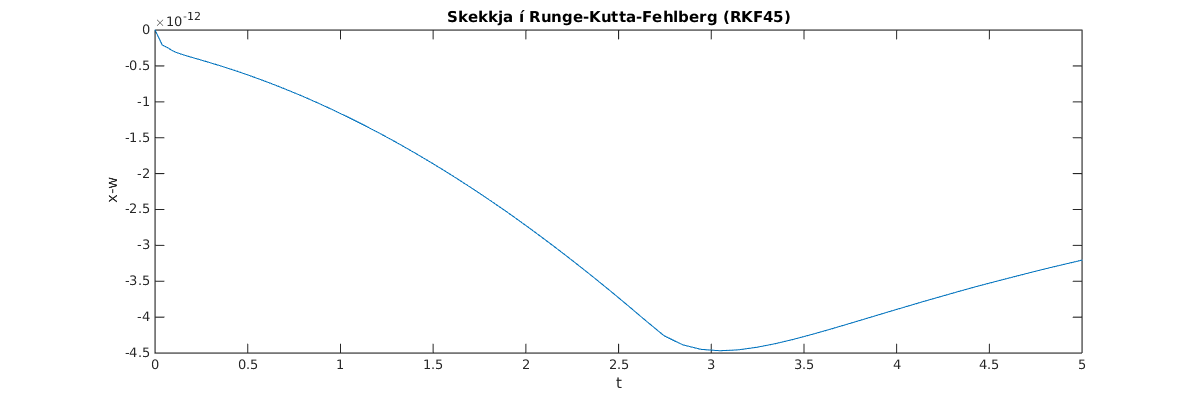
\includegraphics[width=12cm]{./7rkf45.png}}
\mode<article>
{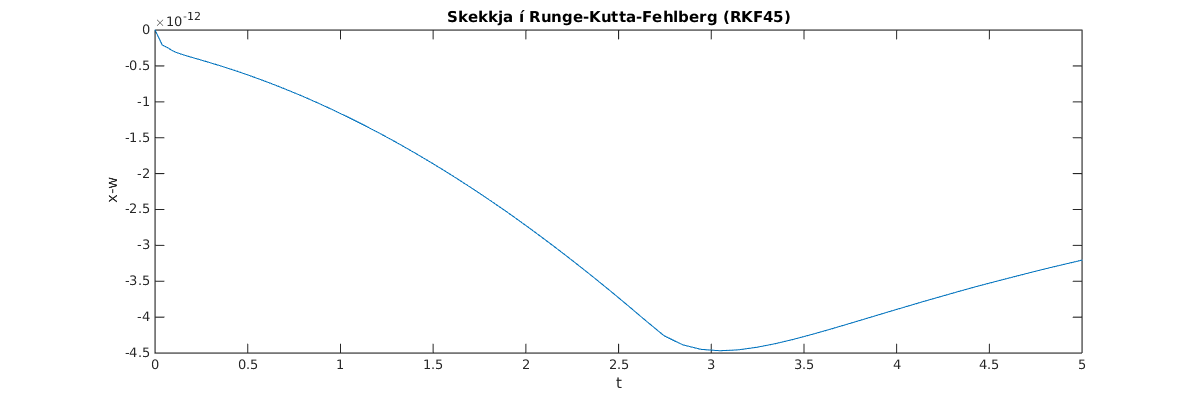
\includegraphics[width=17cm]{./7rkf45.png}}
\end{frame}

\begin{frame}[fragile]{7.7 Runge-Kutte-Fehlberg (RKF45) prófuð, frh.}

Hér á undan þá notðum við þolmörkin $10^{-10}$ sem skilaði okkur 103 misstórum tímagildum
á bilinu $[0,5]$.
Svona getum við teiknað upp stærðina á tímaskrefunum.
\begin{verbatim}
>> plot(t(2:end)-t(1:end-1),'*')
\end{verbatim}
\mode<presentation>
{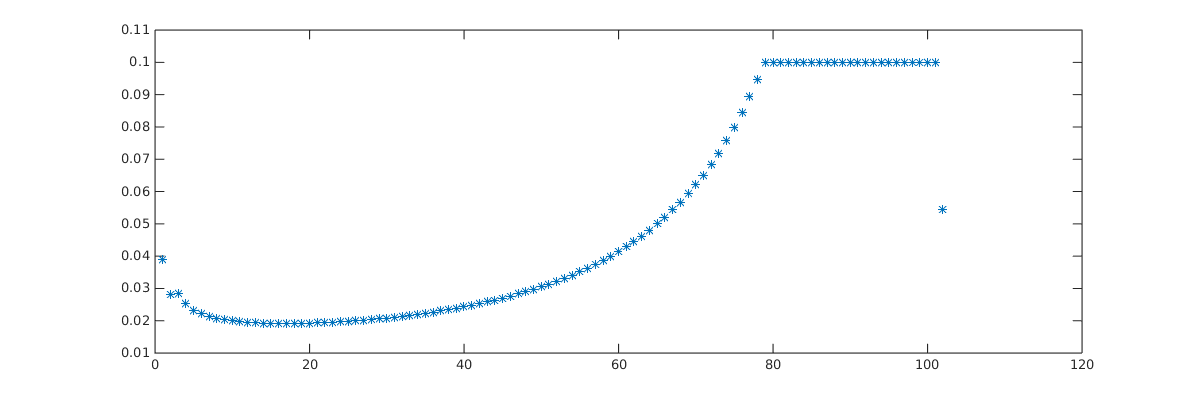
\includegraphics[width=12cm]{./7rkf45t.png}}
\mode<article>
{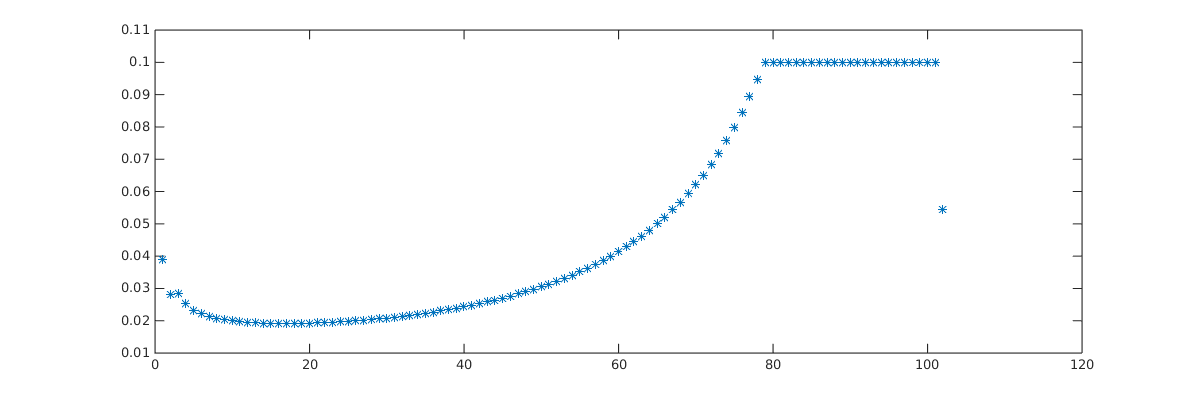
\includegraphics[width=17cm]{./7rkf45t.png}}
\end{frame}



% \begin{frame}{7.7 Nánari útfrærsla á breytilegri skrefstærð} 
% Lesið vandlega grein 7.7 í kennslubókinni þar sem þessu öllu er lýst.
% 
% \pause
% \smallskip
% Í Heimaverkefni II notum við Runge-Kutta-Verner-aðferðina, 
% RKV56.    Þeim er lýst í smáatriðum á bl. 614-15
% 
% \pause
% \smallskip
% Þar er unnið með 5.~og 6.~stigs nálganir sem þýðir að 
% $\alpha_1=5$ og $\alpha_2=6$.  Formúlan fyrir hlutfallinu
% $q$ er
% $$
% q=\bigg(\dfrac{TOL}{2|\varepsilon|}\bigg)^{\frac 15}.
% $$
% 
% \pause
% \smallskip
% Einhverjar takmarkanir þurfa að vera á tölunni $q$, til dæmis
% $$
% 0.1\leq q\leq 4.0.
% $$
% \end{frame}


\begin{frame}{7.5 Fjölskrefaaðferðir} 
Þær aðferðir sem við höfum séð eiga allar sameiginlegt að ákvarða
nálgunargildi $w_{n}$ aðeins út frá gildinu $w_{n-1}$ næst á undan. Hægt
er að nota fleiri gildi $w_{n-1}$, $w_{n-2}$, $\ldots$ og fá þannig betri
nákvæmni, en aðferðirnar verða að sama skapi flóknari í notkun. 

\pause
\smallskip
Eins og alltaf höfum við verkefnið 
\begin{equation*}
  \left\{
    \begin{array}{l}
      x'(t) = f(t,x(t)) \\
      x(t_0) = w_0
    \end{array}
  \right.
\end{equation*}
og viljum nálga gildi lausnarinnar $x$ á bili $[a,b]$ þar sem $a =
t_0$ eða $b = t_0$. Látum $t_0$, $t_1$, $\ldots$, $t_n$ vera skiptingu
á bilinu $[a,b]$ og gerum til einföldunar ráð fyrir að hún hafi jafna
billengd $h=t_{j} - t_{j-1}$ fyrir $j= 1, \ldots, n$. 
\end{frame}


\begin{frame}{7.5 $k$-skrefa  Adams-Bashforth aðferð} 
Við vitum að lausnin $x$ uppfyllir
\begin{equation*}
  x(t_{n}) - x(t_{n-1}) = 
  \int\limits_{t_{n-1}}^{t_n} f(t,x(t)) \, dt 
\end{equation*}

\pause
Skrifum nú
\begin{equation*}
  f(t,x(t)) = P_{k-1}(t) + R_{k-1}(t)
\end{equation*}
þar sem
\begin{equation*}
  P_{k-1}(t) = \sum\limits_{j=1}^k f(t_{n-j},x(t_{n-j})) \cdot
  \ell_{k-1,j}(t)
\end{equation*}
er brúunarmargliðan gegnum punktana $(t_{n-k},x(t_{n-k}))$,
$(t_{n+1-k},x(t_{n+1-k}))$, $\ldots$, $(t_{n-1},x(t_{n-1}))$,
þ.e.~gegnum síðustu $k$ punkta á undan $(t_n,x(t_n))$. 

Þetta eru $k$ punktar og því er aðferðin kölluð $k$-skrefa
aðferð. 
\end{frame}


\begin{frame}{7.5 $k$-skrefa  Adams-Bashforth aðferð} 
Munum að til er  $\xi$ þannig að 
\begin{equation*}
  R_{k-1}(t) = \frac{f^{(k)}(\xi,x(\xi))}{k!}
  \prod\limits_{j=1}^m (t-t_{n-j}).
\end{equation*}
Við nálgum nú heildið af $f$ yfir bilið 
$[t_{n-1},t_n]$ með heildi $P_{k-1}$ og fáum
\begin{equation*}
  w_{i+1} = w_i +
  \int\limits_{t_i}^{t_{i+1}} P_{k-1}(t) \, dt
\end{equation*}
og með beinum  útreikningum má sjá að skekkjan í þessari nálgun er 
$O(h^{k+1})$.  Þessir útreikninga flækjast auðvitað eftir því sem 
$k$ stækkar.
\end{frame}


\begin{frame}{7.5 $k$-skrefa  Adams-Bashforth aðferð, upphafið} 
Augljóslega getum við ekki notað $k$ skrefa Adams-Bashforth aðferðir
um leið og við sjáum upphafsgildisverkefni, því við þurfum $k$
ágiskunargildi $w_0, w_1, \ldots, w_{k-1}$ til að byrja að nota
aðferðina. Þessi gildi má fá með hverri sem er af aðferðunum sem við
höfum séð hingað til. 

\pause
\smallskip
Ákveðin sértilfelli Adams-Bashforth aðferðanna eru meira notuð en
önnur, það eru tveggja, þriggja og fjögurra skrefa
aðferðirnar. Áhugasömum verður ekki skotaskuld úr að leiða út
formúlurnar fyrir þær, en við birtum bara niðurstöðurnar. 

\pause
\smallskip
Til styttingar skilgreinum við  $f_j = f(t_j,w_j)$.
\end{frame}


\begin{frame}{7.5 Tveggja skrefa Adams-Bashforth-aðferð} 
Þegar gildin $w_{n-1}$
og $w_{j-2}$ hafa verið fundin fæst næsta með 
\begin{equation*}
  w_{n} = w_{n-1} + h\big(\tfrac 32 f_{n-1} - \tfrac 12 f_{n-2}\big)
\end{equation*}
og skekkjan í nálguninni er $O(h^3)$. 
\end{frame}


\begin{frame}{7.5 Forrit fyrir tveggja skrefa Adams-Bashforth-aðferð} 
Aðferðin er útfærð í forritinu hér að neðan; það skýrir sig að mestu
sjálft en við skulum taka eftir 
þrennu:  

\pause
\smallskip
(i) Við krefjumst þess að notandinn gefi nálgunargildi á
{\tt x(t(2))}, þetta gerum við því til eru margar mismunandi aðferðir
til að fá slíkt gildi og þær henta mis vel hverju sinni. 

\pause
\smallskip
(ii) Við gerum ekki sérstaklega ráð fyrir að jafnt bil sé á milli
stakanna í vigrinum {\tt t} þó við höfum gert það hingað til. Það var
aðeins gert til að einfalda útreikninga; aðferðin virkar nákvæmlega
eins ef það er ekki jafnt bil á milli stakanna, svo sjálfsagt er að
forrita hana þannig. 

\pause
\smallskip
(iii) Við lágmörkum fjölda skipta sem við reiknum gildi {\tt f} með að
geyma alltaf gildið frá síðustu ítrun og nota það aftur, þetta getur
sparað nokkurn tíma í útreikningum ef {\tt f} er flókið fall. 
\end{frame}


\begin{frame}[fragile]{7.5 Forrit fyrir tveggja skrefa Adams-Bashforth-aðferð} 
\begin{verbatim}
function w = adams_bashforth_2(f,t,x1,x2)
%   w = adams{_}bashforth{_}2(f,t,x1,x2)
% Nálgar lausn upphafsgildisverkefnisins
%   x' = f(t,x)
%   x(t(1)) = x1
% í punktunum í t með 2ja þrepa Adams-Bashforth aðferð.
% Stakið x2 er nálgunargildi á x(t(2)).

N = length(t);  M = length(x1); w = zeros(M,N);
% Upphafsstillum gildi f(t,x) og w
fx1 = f(t(1),x1); fx2 = f(t(2),x2);
w(:,1) = x1; w(:,2) = x2;
for i=3:N
  % Reiknum nálgunargildi
  h = t(i)-t(i-1);
  w(:,i) = w(:,i-1) + (h/2)*(3*fx2 - fx1);
  fx1 = fx2; fx2 = f(t(i),w(:,i));
end
\end{verbatim}
\end{frame}


\begin{frame}{7.5 Þriggja skrefa Adams-Bashforth} 
Gefin $w_{n-1}$, $w_{n-2}$ og $w_{n-3}$ fæst næsta nálgunargildi með
\begin{equation*}
  w_{n} = w_{n-1} + {h}(\tfrac{23}{12} f_{n-1} - \tfrac {16}{12}
  f_{n-2} + \tfrac 5{12} f_{n-2})
\end{equation*}
og staðarskekkjan er $O(h^4)$
\end{frame}


\begin{frame}{7.5 Fjögurra skrefa Adams-Bashforth} 
Þegar við þekkjum $w_{n-1}$, $w_{n-2}$, $w_{n-3}$ og $w_{n-4}$ 
reiknum við næsta gildi með
\begin{equation*}
  w_{n} = w_{n-1} + h\big(\tfrac{55}{24}f_{n-1} - \tfrac{59}{24}f_{n-2} + 
\tfrac {37}{24}f_{n-3} -\tfrac 9{24}f_{n-4}\big)
\end{equation*}
og skekkjan í nálguninni er $O(h^5)$.
\end{frame}


\begin{frame}{7.6  Greining á samleitni og stöðugleika} 
Lítum aftur á upphafsgildisverkefnið okkar
$$
\begin{cases}
  x'(t)=f(t,x(t)),\\
x(t_0)=w_0.
\end{cases}
$$
Við hugsum okkur að nálgun sé fundin í tímapunktunum
$$a=t_0<t_1<t_2<\cdots<t_N=b.$$

\pause
\smallskip
Við táknum nálgunargildi  á $x(t_j)$ með $w_j$. 
Það er gefið með 
$$
w_n=w_{n-1}+h_n\varphi(f,t_{0},\dots,t_n,w_{0},\dots,w_{n})
$$
þar sem fallið $\varphi(f,t_{0},\dots,t_n,w_{0},\dots,w_{n})$
er skilgreint með einhverjum hætti.  

\pause
\smallskip
Við köllum þetta {\it nálgunaraðferðina sem fallið
$\varphi$ gefur af sér.} 
\end{frame}


\begin{frame}{7.6 Nokkur hugtök} 
\begin{block}{Skekkja}
{\it Skekkja} (e.~error) eða  {\it heildarskekkja} 
(e.~total error) í nálgun
á $x(t_n)$ með $w_n$ er 
$$
e_n=x(t_n)-w_n.
$$
\pause
{\it Staðarskekkja} (e.~local truncation error)
nálgunaraðferðarinnar við tímann $t_n$ er
$$
\tau_n=\dfrac{x(t_n)-x(t_{n-1})}{h_n}
-\varphi(f,t_{0},\dots,t_n,x(t_{0}),\dots,x(t_{n}))
$$
Munið að hér er {\it rétta lausnin} sett inn í 
nálgunaraðferðina.
\end{block}
\end{frame}


\begin{frame}{7.6 Samleitni, samræmi og stöðugleiki} 
\begin{block}{Samleitni}  Hugsum okkur nú að fjöldi tímapunktanna 
$N$ stefni á óendanlegt. Við segjum að nálgunaraðferðin $\varphi$
sé {\it samleitin} ef 
$$
\lim_{N\to \infty} \max\limits_{1\leq n\leq N} |e_n|=0
$$
þar sem $e_n=x(t_n)-w_n$ táknar skekkjuna í $n$-ta tímaskrefinu. 
\end{block}
\pause
\begin{block}{Samræmi}
Við segjum að nálgunaraðferðin $\varphi$
{\it samræmist} upphafsgildisverkefninu ef um sérhvern tímapunkt
$t_{n-1}$  gildir að 
\begin{multline*}
\lim_{h_n\to 0}\tau_n\\
=\lim_{t_n\to t_{n-1}}\bigg(\dfrac{x(t_n)-x(t_{n-1})}{t_n-t_{n-1}}
-\varphi(f,t_{0},\dots,t_n,x(t_{0}),\dots,x(t_{n}))\bigg)
=0  
\end{multline*}
\end{block}
\end{frame}


\begin{frame}{7.6 Samræmi endurbættu Euler-aðferðarinnar} 
Munum að endurbætta Euler-aðferðin er
$$
  w_n=w_{n-1}+h_nf(t_{n-1}+\tfrac 12 h_n,w_{n-1}+\tfrac 12 hf(t_{n-1},w_{n-1}))
$$
sem gefur staðarskekkjuna
\begin{multline*}
\tau_n=\dfrac{x(t_{n-1}+h_n)-x(t_{n-1})}{h_n}\\
-f(t_{n-1}+\tfrac 12 h_n,x(t_{n-1})+\tfrac 12 h_nf(t_{n-1},x(t_{n-1}))).
  \end{multline*}
\pause
Nú hugsum við okkur að $t_{n-1}$ sé haldið föstu og látum billengdina
$h_n=t_n-t_{n-1}$ stefna á $0$.  Þá fæst
$$
  \lim_{h_n\to 0} \tau_n= x'(t_{n-1})-f(t_{n-1},x(t_{n-1}))=0
$$
Þetta segir okkur að endurbætta Euler-aðferðin {\bf samræmist} 
upphafsgildisverkefninu.
\end{frame}


\begin{frame}{7.6 Samræmi beinna eins skrefs aðferða} 
Þessi röksemdafærla alhæfist á allar beinar eins skrefs aðferðir, því
staðarskekkja þeirra er 
$$
\tau_n=\dfrac{x(t_{n-1}+h_n)-x(t_{n-1})}{h_n}
-\varphi(f,t_{n-1},t_{n-1}+h_n,x(t_{n-1}))
$$
\pause
Nú er eðlilegt að gefa sér að $\varphi$ sé samfellt fall og
þá verður markgildið af staðarskekkjunni
\begin{multline*}
x'(t_{n-1})-\varphi(f,t_{n-1},t_{n-1},x(t_{n-1}))\\
=f(t_{n-1},x(t_{n-1}))-\varphi(f,t_{n-1},t_{n-1},x(t_{n-1})).
\end{multline*}
Eins skrefs aðferðin sem fallið $\varphi$ gefur af sér er því 
stöðug ef og aðeins ef 
$$
\varphi(f,t_{n-1},t_{n-1},x(t_{n-1}))
=f(t_{n-1},x(t_{n-1})).
$$
\end{frame}


\begin{frame}{7.6 Stöðuleiki} 
Gerum nú ráð fyrir að upphafsgildinu $w_0$ sé breytt í $\tilde w_0$ og
að $\tilde x(t)$ uppfylli
$$
\begin{cases}
  \tilde x'(t)=f(t,\tilde x(t)),\\
\tilde x(t_0)=\tilde w_0.
\end{cases}
$$
Lítum síðan á tilsvarandi nálgunarrunu
$$
\tilde w_n=\tilde w_{n-1}+h_n\varphi(f,t_0,\dots,t_n,\tilde
w_0,\dots,\tilde w_n).
$$
\pause
\begin{block}{Skilgreining}
Við segjum að nálgunaraðferðin sem $\varphi$ gefur af sér 
sé {\it stöðug} ef til er fall $k(t)>0$ þannig að
$$
|\tilde w_n-w_n|\leq k(t_n)|\tilde w_0-w_0|, \qquad n=1,2,3\dots.
$$
\end{block}
\end{frame}


\begin{frame}{7.6 Lipschitz-samfelldni} 
Rifjum nú upp að við gerum ráð fyrir að fallið $f(t,x)$ sé skilgreint
á svæði $D$ sem inniheldur 
$$
\{(t,x)\in \R^2 \, ;\, a\leq t\leq b, x\in \R\}.
$$

\pause
\smallskip
Við segjum að $f$ sé {\it Lipschitz samfellt á $D$ með tilliti til
  $x$} ef til er fasti $C_f$ þannig að 
$$
|f(t,x)-f(t,y)|\leq C_f|x-y|, \qquad x,y\in \R.
$$
Hugsum okkur að $\varphi(f,s,t,x)$ sé fall sem gefur af sér beina eins
skrefs nálgunaraðferð fyrir upphafsgildisverkefnið $x'(t)=f(t,x(t))$
með $x(t_0)=w_0$.  

\pause
\smallskip
Við segjum að $\varphi$ sé {\it Lipschitz-samfellt með
tilliti til $x$} ef um sérhvert Lipschitz-samfellt fall $f$, tölur
$s,t\in [a,b]$ og $x,y\in \R$ gildir að til er fasti $L_\varphi$
þannig að
$$
|\varphi(f,s,t,x)-\varphi(f,s,t,y)|\leq L_\varphi|x-y|, \qquad x,y\in \R.
$$ 
\end{frame}


\begin{frame}{7.6 Setning um stöðugleika og samleitni} 
Gefum okkur jafna skiptingu á tímabilinu $[a,b]$,
$t_n=a+nh$, þar sem $n=0,1,2,\dots,N$ og $h=(b-a)/N$.

\pause
\smallskip
Ef fallið $\varphi$ er Lipschitz-samfellt með tilliti til $x$ 
með Lipschitz-fastann
$L_\varphi$, þá gildir:
  \begin{enumerate}
  \item[(i)] Eins skrefs aðferðin sem $\varphi$ gefur af sér
er stöðug,
$$
|\tilde w_n-w_n|\leq e^{L_\varphi(t_n-a)}|\tilde w_0-w_0|, \qquad
n=1,2,3,\dots. 
$$
  \item[(ii)] Ef til eru fastar $c$ og $p$ þannig að staðarskekkjan
    uppfyllir $|\tau_n|\leq c\, h^p$, fyrir öll $n=1,2,3,\dots$ og
    $h\in ]0,h_0]$, þá er aðferðin samleitin og við höfum
$$
|e_n|=|x(t_n)-w_n|\leq \dfrac{ch^p}{L_\varphi}
\bigg(e^{L_\varphi(t_n-a)}-1\bigg).
$$ 
  \end{enumerate}
\end{frame}


\begin{frame}{Kafli 7: Fræðilegar spurningar}
  \begin{enumerate}
  \item Hvernig er hægt að skrifa annars stigs jöfnu
$u''=f(t,u,u')$ sem jafngilt hneppi?
  \item Hvað er {\it bein aðferð} fyrir upphafsgildisverkefni? 
  \item Hvað er {\it óbein aðferð} fyrir upphafsgildisverkefni? 
  \item Hvað er {\it eins skrefs aðferð} fyrir upphafsgildisverkefni? 
  \item Hvað er {\it fjölskrefaaðferð} fyrir upphafsgildisverkefni? 
  \item Hvernig er {\it aðferð Eulers}? 
  \item Hvernig er {\it aðferð Eulers endurbætt}?
  \item Hvað er {\it forsagnar- og leiðréttingaraðferð}?
  \item Hvernig er {\it 2.~stigs Runge-Kutta aðferð}?
  \item Hvernig er {\it 4.~stigs Runge-Kutta aðferð}?
  \item Hvernig er staðarskekkja í nálgunaraðferð fyrir
    upphafsgildisverkefni skilgreind?
  \end{enumerate}
\end{frame}


\begin{frame}{Kafli 7: Fræðilegar spurningar}
  \begin{enumerate}
  \item [12.]  Rökstyðjið að staðarskekkja í aðferð Eulers sé $O(h)$,
    þar sem $h$ er tímaskrefið.
  \item [13.] Hvernig er tveggja skrefa Adams-Bashforth-aðferð.
  \item [14.] Hvað þýðir að nálgunaraðferð fyrir upphafsgildisverkefni
    sé samleitin?
  \item [15.] Hvað þýðir a nálgunaraðferð samræmist upphafsgildisverkefni?
   \end{enumerate}
\end{frame}

\end{document}